% Observed quantities are inserted by scripts/build_report.py.
\documentclass[11pt,a4paper]{article}
\usepackage[margin=1in]{geometry}
\usepackage{fontspec}
\setmainfont{Times New Roman}
\setmonofont{Consolas}[Scale=0.9]
\usepackage{amsmath,amsthm,mathtools}
\usepackage{unicode-math}
\setmathfont{Cambria Math}
\usepackage[expansion=false]{microtype}
\usepackage{graphicx,booktabs,array,tabularx,longtable}
\usepackage{caption,subcaption,enumitem,placeins}
\usepackage{flafter}
\usepackage[hidelinks]{hyperref}
\setlength{\parindent}{1em}
\setlength{\parskip}{0pt}
\setlength{\emergencystretch}{2em}
\clubpenalty=10000
\widowpenalty=10000
\setlength{\tabcolsep}{4pt}
\renewcommand{\arraystretch}{1.12}
\captionsetup{font=small,labelfont=bf}
\renewcommand{\topfraction}{0.9}
\renewcommand{\bottomfraction}{0.8}
\renewcommand{\textfraction}{0.1}
\renewcommand{\floatpagefraction}{0.75}
\setlist{itemsep=0pt,topsep=3pt}
\newcommand{\R}{\mathbb R}
\newcommand{\E}{\mathbb E}
\newcommand{\one}{\mathbf 1}
\newcommand{\OPT}{\operatorname{OPT}}
\newcommand{\ResearchFigure}[4]{%
 \begin{figure}[tbp]\centering
 \includegraphics[width=\linewidth]{figures/#1.pdf}
 \caption{#2}\label{#3}\end{figure}}
\newcolumntype{Y}{>{\raggedright\arraybackslash}X}
\title{An Empirical Study of Certified Feature Selection\\
for Robust Hypothesis Testing}
\author{}
\date{7 October 2026}
\makeatletter
\renewcommand{\maketitle}{%
\begin{center}
{\Large\bfseries\@title\par}\vspace{4pt}
{\small\@date\par}
\end{center}\vspace{2pt}}
\makeatother

\begin{document}
\maketitle
\begin{abstract}
%%OVERVIEW%%
\end{abstract}

\section{Introduction}
Selecting a small set of measurements for hypothesis testing requires both a
selection criterion and a tractable search over feature subsets. We study a
criterion based on two class-conditional Wasserstein uncertainty sets and a
global-cut algorithm derived from the logical-constraint framework of
Bertsimas et al.\ \cite{unified}. The accompanying theory note establishes
integer exactness and valid optimization bounds. Here we evaluate computation
and independent statistical performance.

The study adapts the independent testing and recovery protocol of Wang et
al.\ \cite{wang}, the small-sample robust-testing setting of Xie et al.\
\cite{xie,gao}, and separate downstream fitting as in Swaroop et al.\
\cite{swaroop}. Six selectors share the same data and evaluation models. We
report both favorable and unfavorable outcomes and distinguish minimization of
the empirical robust criterion from usefulness on an unknown population.

\section{Method summary}
\label{sec:method}
Let $\widehat P_k$ be the empirical distribution of class $k\in\{0,1\}$ and
$\mathcal U_k=\{P:W_1(P,\widehat P_k)\le\theta_k\}$, with positive radii and
standardized L1 transport cost. A mask $z$ selects at most $d$ of the $D$
coordinates, and the test score $g$ depends only on $x_{S(z)}$. The target is
\begin{equation}
\OPT=\min_{\substack{z\in\{0,1\}^D\\ \one^\top z\le d}} V(z),\qquad
V(z)=\inf_{g=g(x_{S(z)})}
\left\{\sup_{P_0\in\mathcal U_0}\E_{P_0}\Phi(-g)
      +\sup_{P_1\in\mathcal U_1}\E_{P_1}\Phi(g)\right\},
\label{eq:target}
\end{equation}
where $\Phi(v)=(1+v)_+/2$. A positive score favors class zero. Clipping scores
to $[-1,1]$ gives a randomized probability $\pi_0=(1+g)/2$; consequently $V$
is a sum of classwise errors and $V/2$ is its balanced-average counterpart.
The constant test has risk $B=1$. A test may ignore extra coordinates, so the
search can use the equality $\one^\top z=d$.

For each fixed support, an exact finite linear program returns a feasible
whole-space test and a dual lower certificate. Its coordinate prices satisfy
$0\le w_{kj}\le\lambda_k$, where $\lambda_k$ prices class-$k$ transport.
We compare three binary-equivalent gates:
\begin{equation}
\begin{array}{ll}
\text{Box:}&w_{kj}\le(B/\theta_k)z_j,\\
\text{Triangle:}&\theta_0w_{0j}+\theta_1w_{1j}\le Bz_j,\\
\text{Risk-scaled:}&\theta_0w_{0j}+\theta_1w_{1j}\le\eta z_j.
\end{array}
\label{eq:gates}
\end{equation}
Here $\eta$ bounds the test objective. The box constants bound multipliers on
the constant-test sublevel set; they are not a population-radius assumption.
The risk-scaled dual supplies a convex fraction and hence a global tangent.
The integer master minimizes the accumulated lower model over all
budget-feasible supports. Each new support triggers a complete oracle refit;
the best feasible original test supplies the upper bound $\bar v$, while the
master supplies a global lower bound $\underline v$. Valid bounds satisfy
$\underline v\le\OPT\le\bar v$. A run is declared numerically optimal only
when
\begin{equation}
\bar v-\underline v\le10^{-6}+10^{-5}|\bar v|.
\label{eq:tolerance}
\end{equation}
The primary risk method adds five fractional root rounds. A no-root variant
isolates their computational effect. All variants start from the same marginal
MMD support. The companion note gives the finite reduction, deployment
construction, dual derivations and proofs; Appendix~\ref{app:ratio} describes
the exploratory full-fraction master.

\section{Experimental design}
\label{sec:design}
\subsection{Data and evaluation splits}
The synthetic study uses $D=12$, a three-coordinate signal set and budget
$d=3$. Class zero is standard Gaussian; class one changes only the signal block
as specified in Table~\ref{tab:mechanisms}. Remaining coordinates are independent
standard Gaussian noise. Coordinate positions are shuffled for each seed,
and recovery uses their underlying semantic identities.
\begin{table}[!htbp]
\centering
\caption{Synthetic alternatives before standardization.}
\label{tab:mechanisms}
\begin{tabularx}{\linewidth}{@{}p{24mm}Y@{}}
\toprule
Mechanism & Class-one signal block\\
\midrule
Mean & Shift each coordinate by $0.9$.\\
Variance & Increase each coordinate's standard deviation to $1.8$.\\
Dependence & Standard-normal marginals with equicorrelation $0.65$.\\
Mixture & Add one shared random sign times $1.5$ to all three coordinates.\\
\bottomrule
\end{tabularx}
\end{table}
The dependence alternative has identical marginal distributions, so useful
signal requires joint measurements. The mixture preserves equal means while
changing marginal shape and joint structure.

Each of 30 training seeds provides disjoint selection and downstream-training
samples of 20 observations per class, and 1,000 fresh classification
observations per class. Centering and scaling are fitted on pooled selection
data and frozen for every selector and later split. The primary radii are
$\theta_0=\theta_1=0.25$. Equality testing uses twenty fresh alternative batches
and twenty null batches per seed, each with 40 observations per class; null
groups are both drawn from class zero.

The real-data study uses UCI WDBC (569 records, 30 features) and Ionosphere
(351 records, 34 features), excluding identifiers and labels
\cite{wdbc,ionosphere}. Twenty stratified splits allocate 20 observations per
class to selection and a disjoint 20 to downstream fitting; remaining
observations are held out. The budget and radii match the synthetic study.
Source hashes, class mappings and complete settings are retained in
Appendix~\ref{app:protocol}.

\subsection{Selectors and reproduction scope}
The six budget-matched selectors are global robust-risk selection, fully
refitted robust greedy, marginal MMD screening, Wang additive-MMD with the paper
objective, L1 logistic ranking and seeded random selection. Robust greedy
minimizes the same criterion at each forward step; marginal screening ranks
one-dimensional unbiased RBF MMD. Logistic ranking uses absolute coefficients
from an L1 fit with liblinear and $C=1$. All methods acquire three features.
Known-signal and all-feature supports are separate diagnostics.

The Wang baseline optimizes an additive coordinate kernel under
$\|\omega\|_2=1$ and $\|\omega\|_0\le d$, using the paper's
mean-minus-variance criterion \cite{wang}. Fixed-support weights are globally
fitted; supports are enumerated for $D\le12$ and searched approximately at
larger $D$. The inspected author revision instead maximizes a positive variance
term. We therefore reproduce the paper objective, not that revision's numerical
pipeline. Appendix~\ref{app:baseline} records the coefficients and provenance.

The primary testing evaluation applies the same joint RBF statistic to each
selected support. Wang's separately reported native signed additive statistic
retains its learned weights; its power is not interchangeable with common
support-only power. Both tests freeze parameters before final labels are used.
The multi-population objective of Swaroop et al.\ and the safe union-screening
task of Hanada et al.\ \cite{hanada} do not define equivalent fixed-budget
comparators for these two class-conditional balls.

\subsection{Metrics and uncertainty}
Optimization outcomes include solved fraction, charged time, bounds, absolute
gap, oracle/master time and distinct integer supports. Runs share a 30-second
selection allowance and use \eqref{eq:tolerance}; all failures and time limits
remain in their denominators. The original-run and retry costs are charged
together.

Equality-test power and null rejection use the unbiased joint RBF MMD with a
selection-fitted median bandwidth. With 199 random label permutations, the
plus-one p-value is $(1+\#\{T_{\rm perm}\ge T_{\rm obs}\})/200$, and the level
is $0.05$. Signal recall is $|S\cap T_*|/|T_*|$. Under the equal support and
signal sizes here, precision and F1 equal recall, while FDP and NDP both equal
one minus recall; they are not independent endpoints.

Each support is independently fitted with the same robust envelope test and
RBF SVM ($C=1$; downstream median bandwidth). Prediction is measured by
thresholded balanced error, randomized balanced error, AUC and predictive
cross-entropy. Randomized balanced error is
$\tfrac12[\overline{1-\pi_0(X)}+\overline{\pi_0(Y)}]$; the empirical half-hinge
average is identical. Hard decisions use threshold $0.5$, with ties assigned
to class zero.

Synthetic intervals are 95\% percentile bootstrap intervals from 2,000
resamples of training seeds. Conditional batches are averaged within seed
first, and method differences retain pairing. Real results are mean
$\pm$ repeated-split SD, because records are reused across splits. Complete
metric tables and effective counts appear in Appendix~\ref{app:results}.

\section{Computational results}
\label{sec:computation}
Small comparisons use mean and mixture data at $(D,d)=(8,2),(12,3)$, eight
source atoms per class and ten paired seeds. Scaling uses $D=20,40,80$, budget
three, ten atoms per class and five seeds. Box, triangle, risk without roots and
risk with roots share the objective, warm support and numerical controls;
small cases also use enumeration.
\begin{figure}[tbp]
\centering
\begin{subfigure}{\linewidth}
\centering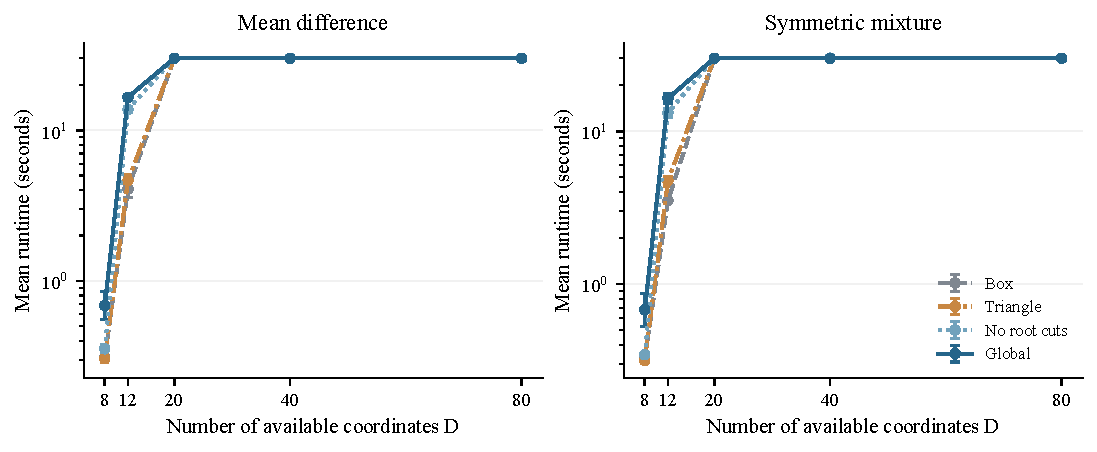
\includegraphics[width=.94\linewidth]{figures/optimization_runtime.pdf}
\caption{Charged selection time; 95\% seed-bootstrap intervals.}
\end{subfigure}
\begin{subfigure}{\linewidth}
\centering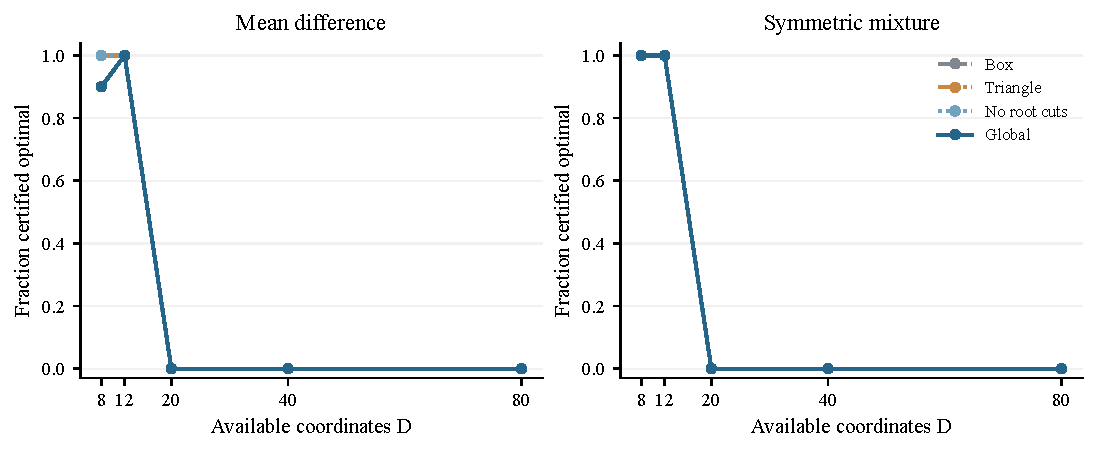
\includegraphics[width=.94\linewidth]{figures/optimization_success.pdf}
\caption{Numerically solved fraction; time limits and failures remain in the denominator.}
\end{subfigure}
\caption{Primary gate comparison under the common selection allowance.
All recorded outcomes are retained. Root and master work and numerical
retries contribute to charged time.}
\label{fig:computation}
\end{figure}
%%COMPUTATIONAL_TABLE%%

\FloatBarrier
\section{Synthetic statistical results}
\label{sec:synthetic}
\subsection{Testing and recovery}
\ResearchFigure{power_and_calibration}
{Common-support two-sample power and null rejection at level $0.05$.
Points average twenty batches within each of thirty training seeds; intervals
resample those seeds.}
{fig:power}{}
\ResearchFigure{support_recovery}
{Signal recall and support stability. Bars show recall with 95\% seed-bootstrap
intervals; diamonds show descriptive pairwise Jaccard stability.}
{fig:recovery}{}
%%STATISTICAL_TABLE%%

\FloatBarrier
\subsection{Prediction and radius sensitivity}
The common robust and SVM classifiers assess support utility on independent
individual observations. Full classifier, ranking and probability-loss
results are in Appendix~\ref{app:results}. We also translate held-out class
observations toward the opposite class along one common downstream-mean
direction of L1 norm one, using magnitudes $0,0.25,0.50$. The worst measured
error is a maximum over these three shifts, rather than a Wasserstein
supremum. A separate source-atom translation has an explicit budget-feasible
coupling and checks the fitted certificate directly.

The predeclared radius analysis refits the procedure at $0.10,0.25,0.50$ for
mean and mixture data on ten seeds. Both selection and downstream robust fitting
change with radius; this comparison does not isolate selection alone.
\ResearchFigure{radius_sensitivity}
{Sensitivity to the three preset radii. Each setting uses the same seed-level
data and independent evaluation protocol; intervals resample ten training
seeds. The primary radius remains $0.25$.}
{fig:radius}{}
%%SENSITIVITY_TABLE%%

\FloatBarrier
\section{Real-data results}
\label{sec:real}
Both datasets use the common budget and independently fitted classifiers.
Global searches are evaluated through their retained supports and recorded
statuses. Table~\ref{tab:real-main} reports predictive variability
over the twenty predefined splits. Selection gaps, stress results and feature
frequencies are provided in Appendix~\ref{app:results}.
%%REAL_TABLE%%

\FloatBarrier
\clearpage
\section{Discussion}
\label{sec:discussion}
The experiments support the optimization formulation but do not establish a
general statistical advantage of the robust criterion. Solved small instances
agree with enumeration, whereas stronger fractional gates did not reduce
elapsed time in this master implementation. Independent testing and
recovery can remain worse even when the empirical risk is optimized to
tolerance. Radius coverage and finite-sample objective choice therefore
require further study.

The empirical head bound applies to its specified Wasserstein balls.
Independently evaluated error can exceed it when population coverage is
unestablished;
the relevant comparison is reported separately from the direct source
feasibility check. The native Wang statistic similarly distinguishes an
end-to-end testing procedure from utility of the same selected support under
a common evaluator.

A separately declared full-fraction master reduced support visits on some
instances without improving elapsed time overall. Appendix~\ref{app:ratio}
reports its paired results and exact binary lift. These exploratory results
motivate improving master solution rather than treating stronger integer
constraints as a runtime guarantee.

The study uses small training samples, moderate computational dimensions,
fixed radii and fixed baseline hyperparameters. Repeated real-data splits
describe variability within two datasets, not performance across independent
populations. No formal multiple-comparison significance claims or clinical
claims are made. All recorded outcomes, original numerical failures and
replay costs are preserved.

\FloatBarrier
\clearpage
\appendix
\section{Protocol and reproducibility}
\label{app:protocol}
\begin{longtable}{@{}p{31mm}p{113mm}@{}}
\caption{Frozen settings. The protocol date is 3 October 2026.}\label{tab:settings}\\
\toprule Experiment & Settings\\\midrule\endfirsthead
\toprule Experiment & Settings\\\midrule\endhead
Statistical & Four alternatives; $D=12$, signal and budget three; seeds
0--29; selection and downstream training 20 per class; classification 1,000
per class; twenty alternative and twenty null batches per seed, each 40 per
class; 199 permutations; radius $0.25$.\\
Small computation & Mean and mixture; $(D,d)=(8,2),(12,3)$; eight atoms per
class; seeds 0--9; four gate/root variants and enumeration.\\
Scaling & Mean and mixture; $D=20,40,80$, $d=3$; ten atoms per class;
seeds 0--4; four gate/root variants.\\
Real data & WDBC and Ionosphere; seeds 0--19; disjoint selection/downstream
samples of 20 per class, remaining records held out; budget three, radius
$0.25$.\\
Radius & Mean and mixture; seeds 0--9; statistical sample sizes; global
risk selection at $0.10,0.25,0.50$.\\
Full-fraction master & Mean and mixture; eight atoms per class; seeds
10--14; $(D,d)=(8,2),(12,3),(20,3)$; tangent versus ratio-plus-tangent;
five root rounds, no core-point selection.\\
Controls & Thirty-second selection allowance, shared warm support,
$10^{-6}$ absolute and $10^{-5}$ relative tolerance; one solver/BLAS thread;
paired data, scaling and evaluation.\\
\bottomrule
\end{longtable}
%%REMEDIATION%%

\subsection{Verification and provenance}
Independent small-instance checks compare the original fixed-support primal
with a source-marginal total-transport dual, enumerate all supports, evaluate
cuts away from their generating support and check whole-space deployment.
They include unequal weights and radii, duplicate observations, empty/full
budgets, analytic curves and smaller logistic-cone cases. Additional checks
cover splitting, kernel coefficients, global weight fitting, permutation
arithmetic, risk normalization and interrupted master bounds.

Each stored run contains its configuration hash, preprocessing, selected
observed and semantic coordinates, splits, bounds, status, timing, fitted
head and test replicates; traces are separate. The final generator checks all
planned keys and compares raw metrics against the public CSV before authoring.
The report manifest hashes its inputs and figure assets. Canonical complete
results remain in
\href{../results/research_20261003/per_trial.csv}{\texttt{per\_trial.csv}} and
\href{../results/research_20261003/summary.json}{\texttt{summary.json}}.
Build revision and the original study's verification/software metadata are
reported with the generated appendix.

\ResearchFigure{evaluation_split}
{Sample roles in a synthetic training seed. Transformations and support use
selection data; downstream fitting and final assessment use separate samples.}
{fig:split-app}{}
\ResearchFigure{gate_mechanism}
{Analytic illustration of gate values and the complete dual fraction. Binary
risk is unchanged; fractional lower models differ. Detailed proofs are in the
companion theory note.}
{fig:gate-app}{}

\section{Baseline fidelity}
\label{app:baseline}
For Wang's paired construction, let
$h_{il,j}=k_j(x_i,x_l)+k_j(y_i,y_l)-k_j(x_i,y_l)-k_j(y_i,x_l)$.
The reproduced mean and row-based variance coefficients are
\begin{equation}
t=\frac1{n(n-1)}\sum_{i\ne l}h_{il},\qquad
r_i=\frac1n\sum_lh_{il},\qquad
\widehat\Sigma=\frac4n\sum_i(r_i-\bar r)(r_i-\bar r)^\top,
\label{eq:wang-coefficients}
\end{equation}
and the criterion is
\begin{equation}
\max_{\|\omega\|_2=1,\ \|\omega\|_0\le d}
t^\top\omega-0.1\,\omega^\top\widehat\Sigma\omega.
\label{eq:wang-criterion}
\end{equation}
On each support an eigendecomposition and secular norm equation give the
global sphere-constrained weight solution, including its hard case.
Coordinate bandwidths follow the inspected revision convention: median
squared cross-class selection distances, factor one, and a constant-column
floor. At larger dimensions the documented forward/swap search is approximate.

The inspected author code \cite{wangcode} maximizes a positive quadratic
variance coefficient, rather than the negative coefficient in
\eqref{eq:wang-criterion}. It also recomputes a cross-class bandwidth using
final labels. Our independently written baseline follows the paper objective
and freezes bandwidths before final testing. Signed weights are retained;
conditional permutation calibration does not require the weighted statistic
to be a positive-definite-kernel MMD. This is a criterion reproduction with
adapted independent evaluation, not a reproduction of the source's tables.
The inspected commit is
\texttt{031f740e9ca6672751145b16de62cfaf731e98de}.
The detailed coefficient fixtures and adaptations are in
\texttt{docs/baseline\_reproduction.md}.

The local source versions are Wang v4 (2024), Xie v1 (2021), Gao v1 (2018),
Swaroop v1 (2025) and Bertsimas v3. Unlicensed author source is not
redistributed. Dataset URLs, DOIs, CC BY 4.0 licenses, hashes, dimensions,
label mappings and excluded columns are in \texttt{docs/data\_sources.json}.

\section{Supplementary results}
\label{app:results}
Synthetic entries are mean [95\% training-seed bootstrap interval]; real
entries are mean $\pm$ split SD. Dashes denote absent or inapplicable values.
Counts and statuses retain unsuccessful outcomes. Redundant half-hinge and
randomized-error aliases are not treated as separate findings.
%%APPENDIX_TABLES%%
\ResearchFigure{population_stress}
{Independent prediction under the preset class-toward-class translations.
The maximum over these shifts is distinct from the direct empirical-ball
source check.}
{fig:stress-app}{}
\ResearchFigure{real_support_frequency}
{Global-selector feature frequencies over twenty repeated splits. These
describe selection stability; the corresponding searches are time-limited
incumbents.}
{fig:frequency-app}{}

\section{Exploratory full-fraction master}
\label{app:ratio}
This supplement was declared after the primary timing observations and before
its own runs. Objective, oracle, warm support, root stage and budget are fixed.
A reusable repaired dual certificate with $\tau>0$ gives
\begin{equation}
V(z)\ge f_c(z)=\frac{v}{\tau+\widehat\mu^\top z},
\qquad 0\le v\le\mathcal H(\widehat\Gamma).
\label{eq:ratio-app}
\end{equation}
Dividing its masses and prices by the denominator restores normalization at
any new support. For a feasible original-test bound $U$, shared products
$y_j=\eta z_j$ have the exact binary representation
\begin{equation}
\begin{gathered}
0\le\eta\le U,\quad0\le y_j\le Uz_j,\quad
y_j\le\eta,\quad y_j\ge\eta-U(1-z_j),\\
v\le\tau\eta+\widehat\mu^\top y,\qquad
\one^\top y=d\eta.
\end{gathered}
\label{eq:lift-app}
\end{equation}
An original optimum with $\eta=\OPT$, $y=\OPT z$ remains feasible, preserving
the global bound. The master retains affine floors as well: the product
relaxation at fractional masks need not dominate a matched tangent, even
though the full fraction does. The incumbent level row
$\widehat\mu^\top z\ge v/U-\tau$ is already implied by \eqref{eq:lift-app}.
Zero-scale and zero-numerator certificates are omitted; a feasible zero-risk
test proves optimality by nonnegativity. The companion note derives these
claims, actual-scale tangents and numerical margins in detail.

\ResearchFigure{ratio_supplement}
{Separately declared paired full-fraction comparison. Seeds 10--14 are used
within this suite; primary-suite timings are not substituted. Both variants
retain failures and limits in their solved fraction.}
{fig:ratio-app}{}
%%RATIO_TABLE%%

\FloatBarrier
\clearpage
\begin{thebibliography}{9}
\bibitem{unified} D. Bertsimas, R. Cory-Wright, and J. Pauphilet.
\emph{A Unified Approach to Mixed-Integer Optimization Problems with Logical
Constraints}.
\href{https://arxiv.org/abs/1907.02109}{arXiv:1907.02109v3}.
\bibitem{xie} L. Xie, R. Gao, and Y. Xie.
\emph{Robust Hypothesis Testing with Wasserstein Uncertainty Sets}. 2021.
\href{https://arxiv.org/abs/2105.14348}{arXiv:2105.14348}.
\bibitem{gao} R. Gao, L. Xie, Y. Xie, and H. Xu.
\emph{Robust Hypothesis Testing Using Wasserstein Uncertainty Sets}. 2018.
\href{https://arxiv.org/abs/1805.10611}{arXiv:1805.10611}.
\bibitem{wang} J. Wang, S. S. Dey, and Y. Xie.
\emph{Variable Selection for Kernel Two-Sample Tests}.
2024. \href{https://arxiv.org/abs/2302.07415}{arXiv:2302.07415v4}.
\bibitem{wangcode} \emph{MMDVar\_Selection}. Source code repository.
\href{https://github.com/WalterBabyRudin/MMDVar_Selection}
{WalterBabyRudin/MMDVar\_Selection}; inspected commit stated in
Appendix~\ref{app:baseline}.
\bibitem{swaroop} M. Swaroop, T. Krishnamurti, and B. Wilder.
\emph{Distributionally Robust Feature Selection}. In \emph{Advances in
Neural Information Processing Systems}, 2025.
\href{https://arxiv.org/abs/2510.21113}{arXiv:2510.21113}.
\bibitem{hanada} H. Hanada, S. Akahane, N. Hashimoto, S. Takeno, and I. Takeuchi.
\emph{Safe Distributionally Robust Feature Selection under Covariate Shift}.
2026. \href{https://arxiv.org/abs/2603.16062}{arXiv:2603.16062}.
\bibitem{wdbc} UCI Machine Learning Repository.
\emph{Breast Cancer Wisconsin (Diagnostic)}.
\href{https://doi.org/10.24432/C5DW2B}{DOI:10.24432/C5DW2B}.
\bibitem{ionosphere} UCI Machine Learning Repository. \emph{Ionosphere}.
\href{https://doi.org/10.24432/C5W01B}{DOI:10.24432/C5W01B}.
\end{thebibliography}
\end{document}
